% question 2
\section{Question 2}

\paragraph{(a)} The bode diagram indicates that close-loop system attenuates signals with frequency higher than $4.5$ Hz and delay output signal with respect to input. Thus, response of close-loop system will present lower oscillations. Figure \ref{fig:q2_mano} describes a sketch of response of close-loop system. 

\begin{figure}[h!]
\centering
\includegraphics{images/question2/q2_a_mano.pdf}
\caption{Sketch of response of close-loop system.}
\label{fig:q2_mano}
\end{figure}

\paragraph{(b)} Considering input signal
\begin{equation*}
r(t)=1\sin{(2 \pi 0.1 t)} + 0.5\sin{(2 \pi t)} + 0.2\sin{(2 \pi 10 t)},
\label{eq:q2a_input}
\end{equation*}
the output signal will be
\begin{equation*}
y(t) = 1\sin{(0.628 t + 0 \textrm{ rad})} + 0.48\sin{(6.28 t - 0.262 \textrm{ rad})} + 0.0796\sin{(62.8 t-1.08 \textrm{ rad})},
\end{equation*}

\begin{figure}[h!]
\centering
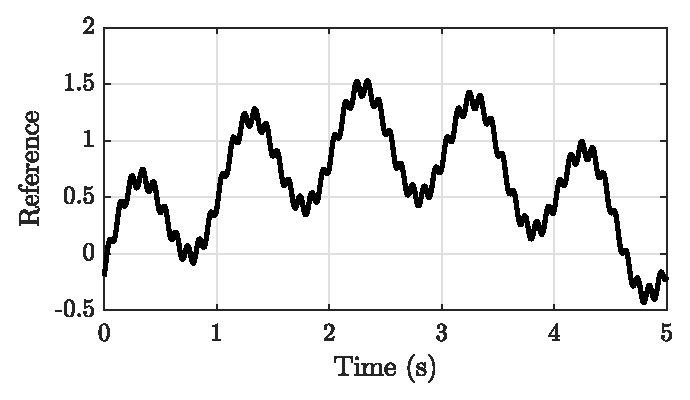
\includegraphics{images/question2/act_2a.eps}
\caption{Response of the close-loop system with input \eqref{eq:q2a_input}.}
\end{figure}
